\documentclass[11pt]{article}
\usepackage[a4paper,margin=1.8cm]{geometry}
\usepackage{tikz}
\usepackage{amsmath}
\setcounter{MaxMatrixCols}{10}
\usepackage{amssymb}
\usepackage{xcolor}
\pagestyle{empty}

\begin{document}
\section*{$S=\{0,1,2,4,6\}$, $m=5$, $t=7$}
\begin{center}
$\mathbf{FACET}$
\end{center}
$\left\lfloor t/2\right\rfloor=3$
\quad\quad
$J=\{1,2,3\}$
\quad\quad
$N=3$
\quad\quad
$\operatorname{rank}(Y^{+})=3$
\quad\quad
$\text{mode}=\text{lifted}$
\quad\quad
$\text{rhs}=2$

\begin{center}
\smallskip Complete graph on $V$, with vertices in $S$ and edges in $E(S)$ highlighted in red. $|E(S)|=10$

\begin{minipage}[t]{0.31\textwidth}
\centering
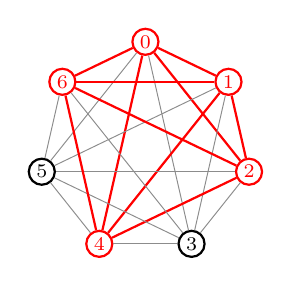
\begin{tikzpicture}[
  thick,
  baseline=(current bounding box.north),
  vertex/.style={circle,draw,inner sep=1.2pt,font=\scriptsize},
  svertex/.style={circle,draw=red,text=red,inner sep=1.2pt,font=\scriptsize}
]
  \node[svertex] (v0) at (0.000,1.350) {0};
  \node[svertex] (v1) at (1.055,0.842) {1};
  \node[svertex] (v2) at (1.316,-0.300) {2};
  \node[vertex] (v3) at (0.586,-1.216) {3};
  \node[svertex] (v4) at (-0.586,-1.216) {4};
  \node[vertex] (v5) at (-1.316,-0.300) {5};
  \node[svertex] (v6) at (-1.055,0.842) {6};
  \draw[red] (v0) -- (v1);
  \draw[red] (v0) -- (v2);
  \draw[black!45,line width=0.35pt] (v0) -- (v3);
  \draw[red] (v0) -- (v4);
  \draw[black!45,line width=0.35pt] (v0) -- (v5);
  \draw[red] (v0) -- (v6);
  \draw[red] (v1) -- (v2);
  \draw[black!45,line width=0.35pt] (v1) -- (v3);
  \draw[red] (v1) -- (v4);
  \draw[black!45,line width=0.35pt] (v1) -- (v5);
  \draw[red] (v1) -- (v6);
  \draw[black!45,line width=0.35pt] (v2) -- (v3);
  \draw[red] (v2) -- (v4);
  \draw[black!45,line width=0.35pt] (v2) -- (v5);
  \draw[red] (v2) -- (v6);
  \draw[black!45,line width=0.35pt] (v3) -- (v4);
  \draw[black!45,line width=0.35pt] (v3) -- (v5);
  \draw[black!45,line width=0.35pt] (v3) -- (v6);
  \draw[black!45,line width=0.35pt] (v4) -- (v5);
  \draw[red] (v4) -- (v6);
  \draw[black!45,line width=0.35pt] (v5) -- (v6);
\end{tikzpicture}
\end{minipage}
\par\smallskip Jumps in $E(S)$: $J=\{1,2,3\}$
\par $a_\ell=\bar{\kappa}(\ell,S,m)=\min\{\kappa(\ell,S),\binom{|S|}{2}-d_m(|S|)\}$
\par $\binom{|S|}{2}-d_m(|S|)=\binom{5}{2}-d_{5}(5)=10-9=1$
\par $a=\left(1,1,1\right)$
\par $a^\top y = y_{1} + y_{2} + y_{3} \le d_m(|S|)+\sum_{\ell\in J} a_\ell-\binom{|S|}{2}=9+3-10=2$
\end{center}

Each drawing below is a circulant graph $G_{L}$ for a non-empty $L\subseteq J$ with edges $E(L)=\{\{i,j\}\mid i,j\in V,\ \min((i-j)\bmod t,\,(j-i)\bmod t)\in L\}$.
For each graph, we show $a^\top y$ for the lifted coefficient vector $a_\ell=\bar{\kappa}(\ell,S,m)$ and put $\textcolor{green!60!black}{\checkmark}$ iff $a^\top y=\mathrm{rhs}$; otherwise $\textcolor{red}{\boldsymbol{\times}}$. The raw overlap $|E(L)\cap E(S)|$ is also shown for reference.
When a checked graph is minimal under single-jump deletion, we append $\textbf{MIN}$ right after the checkmark.
Only graphs that pass the check are shown. 

\noindent
\begin{minipage}[t]{0.31\textwidth}
\centering
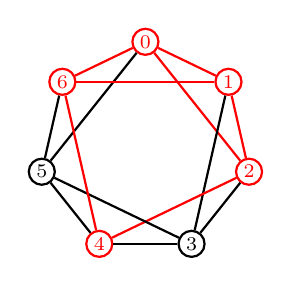
\begin{tikzpicture}[
  thick,  vertex/.style={circle,draw,inner sep=1.2pt,font=\scriptsize},  svertex/.style={circle,draw=red,text=red,inner sep=1.2pt,font=\scriptsize},  baseline=(current bounding box.north)
]
  \node[svertex] (v0) at (0.000,1.350) {0};
  \node[svertex] (v1) at (1.055,0.842) {1};
  \node[svertex] (v2) at (1.316,-0.300) {2};
  \node[vertex] (v3) at (0.586,-1.216) {3};
  \node[svertex] (v4) at (-0.586,-1.216) {4};
  \node[vertex] (v5) at (-1.316,-0.300) {5};
  \node[svertex] (v6) at (-1.055,0.842) {6};
  \draw[red] (v0) -- (v1);
  \draw[red] (v0) -- (v2);
  \draw (v0) -- (v5);
  \draw[red] (v0) -- (v6);
  \draw[red] (v1) -- (v2);
  \draw (v1) -- (v3);
  \draw[red] (v1) -- (v6);
  \draw (v2) -- (v3);
  \draw[red] (v2) -- (v4);
  \draw (v3) -- (v4);
  \draw (v3) -- (v5);
  \draw (v4) -- (v5);
  \draw[red] (v4) -- (v6);
  \draw (v5) -- (v6);
\end{tikzpicture}
\par\smallskip Graph 4
\par $L=\{\textcolor{red}{1},\textcolor{red}{2}\}$
\par $y=\left(\textcolor{red}{1},\textcolor{red}{1},\textcolor{red}{0}\right)$
\par $a^\top y=2\;\;\textcolor{green!60!black}{\checkmark}\;\textbf{MIN}$
\par $|E(L)\cap E(S)|=7$
\end{minipage}\hfill\begin{minipage}[t]{0.31\textwidth}
\centering
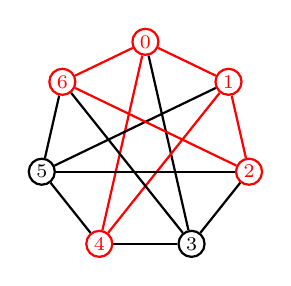
\begin{tikzpicture}[
  thick,  vertex/.style={circle,draw,inner sep=1.2pt,font=\scriptsize},  svertex/.style={circle,draw=red,text=red,inner sep=1.2pt,font=\scriptsize},  baseline=(current bounding box.north)
]
  \node[svertex] (v0) at (0.000,1.350) {0};
  \node[svertex] (v1) at (1.055,0.842) {1};
  \node[svertex] (v2) at (1.316,-0.300) {2};
  \node[vertex] (v3) at (0.586,-1.216) {3};
  \node[svertex] (v4) at (-0.586,-1.216) {4};
  \node[vertex] (v5) at (-1.316,-0.300) {5};
  \node[svertex] (v6) at (-1.055,0.842) {6};
  \draw[red] (v0) -- (v1);
  \draw (v0) -- (v3);
  \draw[red] (v0) -- (v4);
  \draw[red] (v0) -- (v6);
  \draw[red] (v1) -- (v2);
  \draw[red] (v1) -- (v4);
  \draw (v1) -- (v5);
  \draw (v2) -- (v3);
  \draw (v2) -- (v5);
  \draw[red] (v2) -- (v6);
  \draw (v3) -- (v4);
  \draw (v3) -- (v6);
  \draw (v4) -- (v5);
  \draw (v5) -- (v6);
\end{tikzpicture}
\par\smallskip Graph 5
\par $L=\{\textcolor{red}{1},\textcolor{red}{3}\}$
\par $y=\left(\textcolor{red}{1},\textcolor{red}{0},\textcolor{red}{1}\right)$
\par $a^\top y=2\;\;\textcolor{green!60!black}{\checkmark}\;\textbf{MIN}$
\par $|E(L)\cap E(S)|=6$
\end{minipage}\hfill\begin{minipage}[t]{0.31\textwidth}
\centering
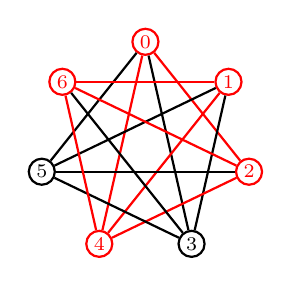
\begin{tikzpicture}[
  thick,  vertex/.style={circle,draw,inner sep=1.2pt,font=\scriptsize},  svertex/.style={circle,draw=red,text=red,inner sep=1.2pt,font=\scriptsize},  baseline=(current bounding box.north)
]
  \node[svertex] (v0) at (0.000,1.350) {0};
  \node[svertex] (v1) at (1.055,0.842) {1};
  \node[svertex] (v2) at (1.316,-0.300) {2};
  \node[vertex] (v3) at (0.586,-1.216) {3};
  \node[svertex] (v4) at (-0.586,-1.216) {4};
  \node[vertex] (v5) at (-1.316,-0.300) {5};
  \node[svertex] (v6) at (-1.055,0.842) {6};
  \draw[red] (v0) -- (v2);
  \draw (v0) -- (v3);
  \draw[red] (v0) -- (v4);
  \draw (v0) -- (v5);
  \draw (v1) -- (v3);
  \draw[red] (v1) -- (v4);
  \draw (v1) -- (v5);
  \draw[red] (v1) -- (v6);
  \draw[red] (v2) -- (v4);
  \draw (v2) -- (v5);
  \draw[red] (v2) -- (v6);
  \draw (v3) -- (v5);
  \draw (v3) -- (v6);
  \draw[red] (v4) -- (v6);
\end{tikzpicture}
\par\smallskip Graph 6
\par $L=\{\textcolor{red}{2},\textcolor{red}{3}\}$
\par $y=\left(\textcolor{red}{0},\textcolor{red}{1},\textcolor{red}{1}\right)$
\par $a^\top y=2\;\;\textcolor{green!60!black}{\checkmark}\;\textbf{MIN}$
\par $|E(L)\cap E(S)|=7$
\end{minipage}
\par\medskip

\noindent\textbf{Matrix Data}
\par $N=3$
\par $a=\left(1,1,1\right)$
\par $\mathrm{rhs}=2$
\par $I=\{4,5,6\}$\quad$Y=\begin{bmatrix}1 & 1 & 0 \\ 1 & 0 & 1 \\ 0 & 1 & 1\end{bmatrix}$
\par $Y^{+}=\begin{bmatrix}1 & 1 & 0 \\ 1 & 0 & 1 \\ 0 & 1 & 1 \\ 1 & 1 & 1\end{bmatrix}$\quad$\operatorname{rank}(Y^{+})=3$
\end{document}
